\documentclass[letterpaper]{article}
\usepackage[ascii]{inputenc}
\usepackage[noenc]{tipa}
\usepackage{tipx}
\usepackage[geometry,weather,misc,clock]{ifsym}
\usepackage{pifont}
\usepackage{eurosym}
\usepackage{amsmath}
\usepackage{wasysym}
\usepackage{amssymb,amsfonts,textcomp}
\usepackage[T3,T1]{fontenc}
\usepackage[english]{babel}
\usepackage{color}
\usepackage{multicol}
\usepackage{array}
\usepackage{hhline}
\usepackage{hyperref}
\usepackage{graphicx}
\graphicspath{ {./images/} }
\hypersetup{colorlinks=true, linkcolor=blue, citecolor=blue, filecolor=blue, urlcolor=blue}
\makeatletter
\newcommand\arraybslash{\let\\\@arraycr}
\makeatother
% Page layout (geometry)
\setlength\voffset{-1in}
\setlength\hoffset{-1in}
\setlength\topmargin{2.54cm}
\setlength\oddsidemargin{2.54cm}
\setlength\textheight{22.86cm}
\setlength\textwidth{16.509998cm}
\setlength\footskip{0.0cm}
\setlength\headheight{0cm}
\setlength\headsep{0cm}
% Footnote rule
\setlength{\skip\footins}{0.119cm}
\renewcommand\footnoterule{\vspace*{-0.018cm}\setlength\leftskip{0pt}\setlength\rightskip{0pt plus 1fil}\noindent\textcolor{black}{\rule{0.25\columnwidth}{0.018cm}}\vspace*{0.101cm}}
% Pages styles
\makeatletter
\newcommand\ps@Standard{
  \renewcommand\@oddhead{}
  \renewcommand\@evenhead{}
  \renewcommand\@oddfoot{}
  \renewcommand\@evenfoot{}
  \renewcommand\thepage{\arabic{page}}
}
\makeatother
\pagestyle{Standard}
\setlength\tabcolsep{1mm}
\renewcommand\arraystretch{1.3}
\title{}
\author{}
\date{2021-04-13}
\begin{document}
\clearpage\setcounter{page}{1}\pagestyle{Standard}
{\centering\bfseries
Design and Analysis of Algorithms
\par}

{\centering\bfseries
DAA432C
\par}

{\centering\bfseries
\ Assignment 2 
\par}

{\centering\bfseries
\ Group - 14 
\par}

{\centering\bfseries
Mukul Mohmare \ \ \ \ \ Anshuman Bharadwaj \ \ \ \ \ \ \ \ \ KishanTripathi
\par}

{\centering\bfseries
\ \ \ \ IIT2019226 \ \ \ \ \ \ \ \ \ \ \ \ \ \ \ \ \ \ \ \ \ \ \ \ \ \ \ IIT2019227
\ \ \ \ \ \ \ \ \ \ \ \ \ \ \ \ \ \ \ \ IIT2019225
\par}


\bigskip

\begin{multicols}{2}
{\bfseries\itshape
Abstract --- Given a string, print the longest repeating subsequence such that the two subsequences don't have same
string character at same position, i.e., any j'th character in the two subsequences shouldn't have the same location
index in the given original string. Solve using dynamic programming.}


\bigskip


\bigskip

I. \ \ \ \ \ \ \ \ \ \ \ \ \ \ \ \ \ \ \ INTRODUCTION


\bigskip

We are given a string we need to find a subsequence which is repeating and is the longest one in the given string.

And we are going to use dynamic programming to solve this question. 

Dynamic programming is a very powerful technique to solve a particular class of problems. It demands very elegant
formulation of the approach and simple thinking and the coding part is very easy. The idea is very simple, If you have
solved a problem with the given input, then save the result for future reference, so as to avoid solving the same
problem again.. shortly \textit{{}'Remember your Past'} :) . \ If the given problem can be broken up into smaller
subproblems and these smaller subproblems are in turn divided in to still-smaller ones, and in this process, if we
observe some overlapping subproblems, then it's a big hint for Dynamic Programming.There are two ways of doing this.

\textbf{1.) Top-Down : }Start solving the given problem by breaking it down. If you see that the problem has been solved
already, then just return the saved answer. If it has not been solved, solve it and save the answer. This is usually
easy to think of and very intuitive. This is referred to as \textbf{\textit{Memoization}}.

\textbf{2.) Bottom-Up} \textbf{:} Analyze the problem and see the order in which the sub-problems are solved and start
solving from the trivial subproblem, up towards the given problem. In this process, it is guaranteed that the
subproblems are solved before solving the problem. This is referred to as \textbf{\textit{Dynamic
}}\textbf{\textit{Programming}}.


\bigskip

\textbf{Subsequence} is a sequence that can be derived from another sequence by deleting some or no elements without
changing the order of the remaining elements. 

Now suppose we choose a string S

\ S = \ {}``ATACTCGGA''

\ Output: ``ATCG''

\ Here we observe that ``ATCG'' is repeating twice \ and is \ the longest among all the repeating sequences in this
string.

\ let's take another example with string S

\ S = ``AABCBDC''

\ Output: ``ABC''

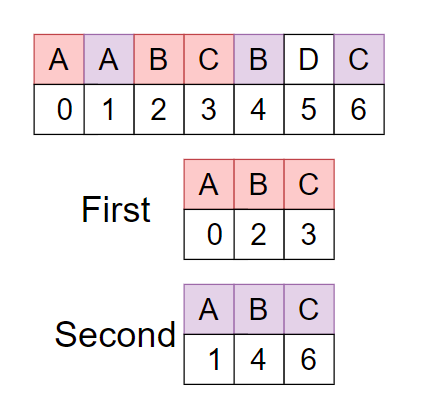
\includegraphics[scale=0.4]{string}

For this example our dynamic programming solution will give output in \ O(n\^{}2) complexity.

Where ,

n =length of given string 

{\bfseries
This report further contains -}

{\bfseries
II. Algorithm Design}

{\bfseries
III. Code And Illustration}

{\bfseries
IV. Algorithm Analysis}

{\bfseries
V. Conclusion}

{\bfseries
VI.References}


\bigskip

{\bfseries
II. ALGORITHM DESIGN}


\bigskip

For this problem , the main idea is to find the subsequence which is repeating \ for the longest length and \textbf{with
the restriction that when both the characters are the same , they shouldn't be on the same index in the two strings. }

We first prepare a table which stores the longest common subsequence \ between the given string and a copy of the same
string but this time we need to keep a check that \ \textbf{when both the characters are the same , they shouldn't be
on the same index in the two strings. }

Now Initialize a resulting string

\ s1 = {\textquotedbl}{\textquotedbl};

Traverse t[][] from bottom right

i = n;

j = n;

while (i {\textgreater} 0 \&\& j {\textgreater} 0)

\{

If this cell is the same as the diagonally adjacent cell just above it, then the same characters are present at str[i-1]
and str[j-1]. Append any of them to string s1.

\ \ \ if (t[i][j] == t[i-1][j-1] + 1)

\ \ \ \{

\ \ \ \ \ s1= s1+ str[i-1];

\ \ \ \ \ i-{}-;

\ \ \ \ \ j-{}-;

\ \ \ \}

Otherwise we move to the side that that gave us maximum result else if (t[i][j] ==

t[i-1][j])

\ \ \ \ i-{}-;

\ \ \ else

\ \ \ \ j-{}-;

\ \}

Since we traverse t[][] from bottom, we get the result in reverse order.

reverse(s1.begin(), res.end());

\ return s1;


\bigskip


\bigskip


\bigskip

III. CODE AND ILLUSTRATION

{\bfseries
Approach -1 Using Tabulation (Bottom Up)}


\bigskip

{\color[rgb]{0.2509804,0.25882354,0.30588236}
\#include {\textless}bits/stdc++.h{\textgreater}}

{\color[rgb]{0.2509804,0.25882354,0.30588236}
using namespace std;}


\bigskip

{\color[rgb]{0.2509804,0.25882354,0.30588236}
string longestRepeatedSubSeq(string str)}

{\color[rgb]{0.2509804,0.25882354,0.30588236}
\{}


\bigskip

{\color[rgb]{0.2509804,0.25882354,0.30588236}
\ \ \ \ int n = str.length();}

{\color[rgb]{0.2509804,0.25882354,0.30588236}
\ \ \ \ int dp[n+1][n+1];}

{\color[rgb]{0.2509804,0.25882354,0.30588236}
\ \ \ \ for (int i=0; i{\textless}=n; i++)}

{\color[rgb]{0.2509804,0.25882354,0.30588236}
\ \ \ \ \ \ \ \ for (int j=0; j{\textless}=n; j++)}

{\color[rgb]{0.2509804,0.25882354,0.30588236}
\ \ \ \ \ \ \ \ \ \ \ \ dp[i][j] = 0;}

{\color[rgb]{0.2509804,0.25882354,0.30588236}
\ \ \ \ for (int i=1; i{\textless}=n; i++)}

{\color[rgb]{0.2509804,0.25882354,0.30588236}
\ \ \ \ \ \ \ \ for (int j=1; j{\textless}=n; j++)}

{\color[rgb]{0.2509804,0.25882354,0.30588236}
\ \ \ \ \ \ \ \ \ \ \ \ if (str[i-1] == str[j-1] \&\& i != j)}

{\color[rgb]{0.2509804,0.25882354,0.30588236}
\ \ \ \ \ \ \ \ \ \ \ \ \ \ \ \ dp[i][j] = \ 1 + dp[i-1][j-1];}

{\color[rgb]{0.2509804,0.25882354,0.30588236}
\ \ \ \ \ \ \ \ \ \ \ \ else}

{\color[rgb]{0.2509804,0.25882354,0.30588236}
\ \ \ \ \ \ \ \ \ \ \ \ \ \ \ \ dp[i][j] = max(dp[i][j-1], dp[i-1][j]);}


\bigskip


\bigskip


\bigskip

{\color[rgb]{0.2509804,0.25882354,0.30588236}
\ \ \ \ string res = {\textquotedbl}{\textquotedbl};}


\bigskip

{\color[rgb]{0.2509804,0.25882354,0.30588236}
\ \ \ \ int i = n, j = n;}

{\color[rgb]{0.2509804,0.25882354,0.30588236}
\ \ \ \ while (i {\textgreater} 0 \&\& j {\textgreater} 0)}

{\color[rgb]{0.2509804,0.25882354,0.30588236}
\ \ \ \ \{}


\bigskip

{\color[rgb]{0.2509804,0.25882354,0.30588236}
\ \ \ \ \ \ \ \ if (dp[i][j] == dp[i-1][j-1] + 1)}

{\color[rgb]{0.2509804,0.25882354,0.30588236}
\ \ \ \ \ \ \ \ \{}

{\color[rgb]{0.2509804,0.25882354,0.30588236}
\ \ \ \ \ \ \ \ \ \ \ res = res + str[i-1];}

{\color[rgb]{0.2509804,0.25882354,0.30588236}
\ \ \ \ \ \ \ \ \ \ \ i-{}-;}

{\color[rgb]{0.2509804,0.25882354,0.30588236}
\ \ \ \ \ \ \ \ \ \ \ j-{}-;}

{\color[rgb]{0.2509804,0.25882354,0.30588236}
\ \ \ \ \ \ \ \ \}}


\bigskip

{\color[rgb]{0.2509804,0.25882354,0.30588236}
\ \ \ \ \ \ \ \ else if (dp[i][j] == dp[i-1][j])}

{\color[rgb]{0.2509804,0.25882354,0.30588236}
\ \ \ \ \ \ \ \ \ \ \ \ i-{}-;}

{\color[rgb]{0.2509804,0.25882354,0.30588236}
\ \ \ \ \ \ \ \ else}

{\color[rgb]{0.2509804,0.25882354,0.30588236}
\ \ \ \ \ \ \ \ \ \ \ \ j-{}-;}

{\color[rgb]{0.2509804,0.25882354,0.30588236}
\ \ \ \ \}}


\bigskip


\bigskip

{\color[rgb]{0.2509804,0.25882354,0.30588236}
\ \ \ \ reverse(res.begin(), res.end());}


\bigskip

{\color[rgb]{0.2509804,0.25882354,0.30588236}
\ \ \ \ return res;}

{\color[rgb]{0.2509804,0.25882354,0.30588236}
\}}


\bigskip

{\color[rgb]{0.2509804,0.25882354,0.30588236}
// Driver Program}

{\color[rgb]{0.2509804,0.25882354,0.30588236}
int main()}

{\color[rgb]{0.2509804,0.25882354,0.30588236}
\{}

{\color[rgb]{0.2509804,0.25882354,0.30588236}
\ \ \ \ string str;}

{\color[rgb]{0.2509804,0.25882354,0.30588236}
\ \ \ \ cin {\textgreater}{\textgreater} str;}

{\color[rgb]{0.2509804,0.25882354,0.30588236}
\ \ \ \ cout {\textless}{\textless} longestRepeatedSubSeq(str);}

{\color[rgb]{0.2509804,0.25882354,0.30588236}
\ \ \ \ return 0;}

{\color[rgb]{0.2509804,0.25882354,0.30588236}
\}}


\bigskip

{\bfseries
Illustration - Approach -1}

Input : String = ``AABCBDC''

Output : ABC

n = string length // 7

Here length of string is 7 

Creating dp table of size 8x8

If String character matches and indexes are different then

dp[i][j] = \ 1 + dp[i-1][j-1];

Else 

dp[i][j] = max(dp[i][j-1] , dp[i-1][j]);

\begin{table}
\raggedright
\begin{tabular}{|m{0.68cm}|m{0.611cm}|m{0.68200004cm}|m{0.788cm}|m{0.68200004cm}|m{0.611cm}|m{0.53900003cm}|m{0.68200004cm}|m{0.544cm}|}

\hline
~
 &
~
 &
{\bfseries a} &
{\bfseries a} &
{\bfseries b} &
{\bfseries c} &
{\bfseries b} &
{\bfseries d} &
{\bfseries c}\\\hline
~
 &
0 &
0 &
0 &
0 &
0 &
0 &
0 &
0\\\hline
{\bfseries a} &
0 &
0 &
1 &
1 &
1 &
1 &
1 &
1\\\hline
{\bfseries a} &
0 &
1 &
1 &
1 &
1 &
1 &
1 &
1\\\hline
{\bfseries b} &
0 &
1 &
1 &
1 &
1 &
2 &
2 &
2\\\hline
{\bfseries c} &
0 &
1 &
1 &
1 &
1 &
2 &
3 &
3\\\hline
{\bfseries b} &
0 &
1 &
1 &
2 &
2 &
2 &
3 &
3\\\hline
{\bfseries d} &
0 &
1 &
1 &
2 &
3 &
3 &
3 &
3\\\hline
{\bfseries c} &
0 &
1 &
1 &
2 &
3 &
3 &
3 &
3\\\hline\end{tabular}

\end{table}
After generating Dp table we initialise an empty string (res=''{}'') to store the ans and print the string

Traverse the dp table in reverse order

Int this case we will traverse from dp[8][8] 

if (dp[i][j] == dp[i-1][j-1] + 1)

\ \ \ \ \ \ \ Then \ \ \ \ res = res + str[i-1];

First character `c' is added to res 

Then character `b' is added and at the last character 'a' is added to res.

Finally reversing the res string and printing the output . 


\bigskip


\bigskip


\bigskip

{\bfseries
Approach-2 }

{\bfseries
Using Recursion with Memoization (Top-Down)}


\bigskip

\#include {\textless}bits/stdc++.h{\textgreater}

using namespace std;

\ int dp[1001][1001];

int longestRepeatedSubSeq(string str,int n,int m)

\{

\ \ \ \ if (dp[n][m]!=0)

\ \ \ \ return dp[n][m];

\ \ \ \ if (n==0{\textbar}{\textbar}m==0)

\ \ \ \ return 0;

\ \ \ \ else if (str[n-1]==str[m-1]\&\& n != m)

\ \ \ \ return dp[n][m]=1+longestRepeatedSubSeq(str,n-1,m-1);

\ \ \ \ else

\ \ \ \ return dp[n][m]=max(longestRepeatedSubSeq(str,n-1,m),longestRepeatedSubSeq(str,n,m-1));


\bigskip


\bigskip


\bigskip


\bigskip

\}


\bigskip


\bigskip

int main()

\{

\ \ \ \ string str;

\ \ \ \ cin {\textgreater}{\textgreater} str;

\ \ \ \ memset(dp,0,sizeof(dp));

\ \ \ \ int n=str.length();

\ \ \ \ longestRepeatedSubSeq(str,n,n);


\bigskip

\ \ \ string res = {\textquotedbl}{\textquotedbl};


\bigskip

\ \ \ \ int i = n, j = n;

\ \ \ \ while (i {\textgreater} 0 \&\& j {\textgreater} 0)

\ \ \ \ \{


\bigskip

\ \ \ \ \ \ \ \ if (dp[i][j] == dp[i-1][j-1] + 1)

\ \ \ \ \ \ \ \ \{

\ \ \ \ \ \ \ \ \ \ \ res = res + str[i-1];

\ \ \ \ \ \ \ \ \ \ \ i-{}-;

\ \ \ \ \ \ \ \ \ \ \ j-{}-;

\ \ \ \ \ \ \ \ \}


\bigskip

\ \ \ \ \ \ \ \ else if (dp[i][j] == dp[i-1][j])

\ \ \ \ \ \ \ \ \ \ \ \ i-{}-;

\ \ \ \ \ \ \ \ else

\ \ \ \ \ \ \ \ \ \ \ \ j-{}-;

\ \ \ \ \}


\bigskip


\bigskip

\ \ \ \ reverse(res.begin(), res.end());


\bigskip


\bigskip

\ \ \ \ cout{\textless}{\textless}res;

\}


\bigskip

\ Illustration - Approach -2 

Same as the previous approach only difference here is we use recursion instead of iteration.

if (dp[n][m]!=0)

\ \ \ \ return dp[n][m];

\ \ \ \ if (n==0{\textbar}{\textbar}m==0)

\ \ \ \ return 0;

\ \ \ \ else if (str[n-1]==str[m-1]\&\& n != m)

\ \ \ \ return dp[n][m]=1+longestRepeatedSubSeq(str,n-1,m-1);

\ \ \ \ else

\ \ \ \ return dp[n][m]=max(longestRepeatedSubSeq(str,n-1,m),longestRepeatedSubSeq(str,n,m-1));


\bigskip

Dp table after recursive calls


\bigskip

\begin{table}
\raggedright
\begin{tabular}{|m{0.68cm}|m{0.611cm}|m{0.68200004cm}|m{0.788cm}|m{0.68200004cm}|m{0.611cm}|m{0.53900003cm}|m{0.68200004cm}|m{0.544cm}|}

\hline
~
 &
~
 &
{\bfseries a} &
{\bfseries a} &
{\bfseries b} &
{\bfseries c} &
{\bfseries b} &
{\bfseries d} &
{\bfseries c}\\\hline
~
 &
0 &
0 &
0 &
0 &
0 &
0 &
0 &
0\\\hline
{\bfseries a} &
0 &
0 &
1 &
1 &
1 &
1 &
1 &
1\\\hline
{\bfseries a} &
0 &
1 &
1 &
1 &
1 &
1 &
1 &
1\\\hline
{\bfseries b} &
0 &
1 &
1 &
1 &
1 &
2 &
2 &
2\\\hline
{\bfseries c} &
0 &
1 &
1 &
1 &
1 &
2 &
3 &
3\\\hline
{\bfseries b} &
0 &
1 &
1 &
2 &
2 &
2 &
3 &
3\\\hline
{\bfseries d} &
0 &
1 &
1 &
2 &
3 &
3 &
3 &
3\\\hline
{\bfseries c} &
0 &
1 &
1 &
2 &
3 &
3 &
3 &
3\\\hline\end{tabular}

\end{table}

\bigskip

{\bfseries
IV. ALGORITHM ANALYSIS}


\bigskip

Time Complexity - Time complexity is the number of operations an algorithm performs to complete its task (considering
that each operation takes the same amount of time). The algorithm that performs the task in the smallest number of
operations is considered the most efficient one in terms of the time complexity.

\ Time Complexity -- O(n\^{}2)

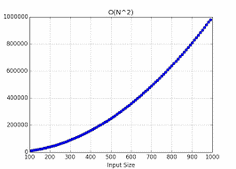
\includegraphics[scale=1]{complexity}


\bigskip

Space Complexity - The space complexity of an algorithm is the amount of memory space required to solve an instance of
the \href{https://en.wikipedia.org/wiki/Computational_problem}{\textcolor[rgb]{0.06666667,0.33333334,0.8}{computational
problem}} as a function of characteristics of the input. It is the memory required by an algorithm until it executes
completely.

Space Complexity -- O(n\^{}2)

\ \ \ \ \ \ \ \ \ \ \ \ \ //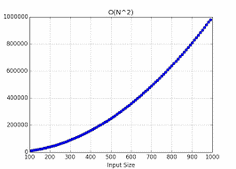
\includegraphics[scale=1]{complexity}

{\bfseries
V. CONCLUSION}

\ Here we have seen booth approaches of dynamic programming to solve this question with great ease . Memoization
approach is really very easy to think and once a recursive solution is framed iterative code is also generated

Using Dynamic programming we solved this problem in quadratic \ complexity which \ proves the efficiency of Dynamic
Programming solution.


\bigskip


\bigskip


\bigskip


\bigskip


\bigskip


\bigskip
\end{multicols}
{\bfseries
VI.REFERENCES}

\bigskip

\ \url{https://www.geeksforgeeks.org/longest-repeated-subsequence/}

\url{https://www.techiedelight.com/longest-repeated-subsequence-problem/}

\url{https://www.geeksforgeeks.org/longest-repeating-subsequence/}

\bigskip


\bigskip


\bigskip


\bigskip
\end{document}
